\documentclass{standalone}

\usepackage{libertinus}
\usepackage[T1]{fontenc}
\renewcommand*\familydefault{\sfdefault}

\usepackage{DejaVuSansMono}

\usepackage{tikz}
\tikzset{every path/.style={semithick}}

\begin{document}
  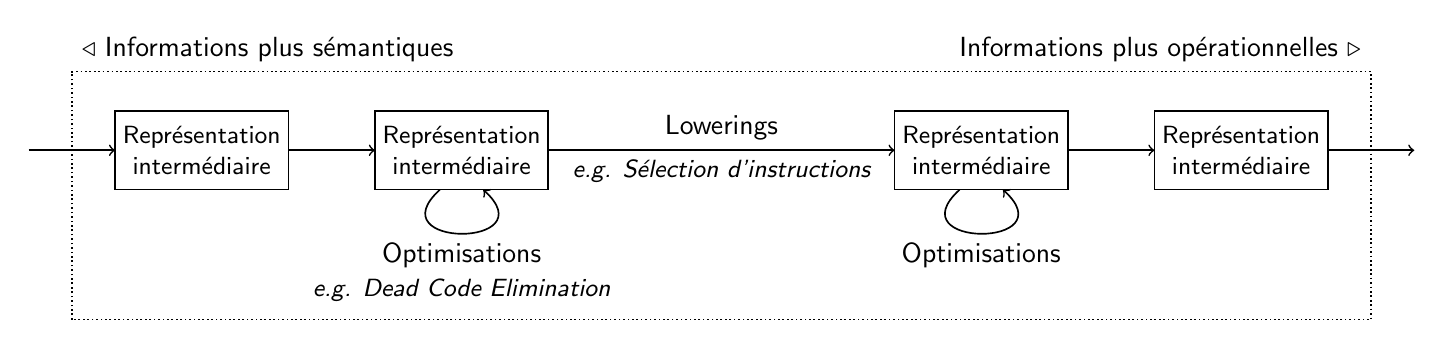
\begin{tikzpicture}[xscale=1.1]
    \draw (0,0) rectangle node[align=center,font=\small] {Représentation \\ intermédiaire} ++(2,1);
    \draw (3,0) rectangle node[align=center,font=\small] {Représentation \\ intermédiaire} ++(2,1);
    \draw (9,0) rectangle node[align=center,font=\small] {Représentation \\ intermédiaire} ++(2,1);
    \draw (12,0) rectangle node[align=center,font=\small] {Représentation \\ intermédiaire} ++(2,1);

    \draw[->] (-1,0.5) -- ++(1,0);
    \draw[->] (2,0.5) -- ++(1,0);
    \draw[->] (5,0.5) -- node[above] {Lowerings} node[below,align=center]
      {\small\it e.g. Sélection d'instructions} ++(4,0);
    \draw[->] (11,0.5) -- ++(1,0);
    \draw[->] (14,0.5) -- ++(1,0);

    \draw[->] (3.75,0) to[out=225, in=315, distance=30] node[below,align=center]
      {Optimisations \\ \small\it e.g. Dead Code Elimination} ++(0.5,0);

    \draw[->] (9.75,0) to[out=225, in=315, distance=30] node[below,align=center]
      {Optimisations} ++(0.5,0);

    \draw[densely dotted] (-0.5,-1.65) rectangle (14.5,1.5);
    \draw (-0.5,1.5) node[above right] {$\triangleleft$ Informations plus sémantiques};
    \draw (14.5,1.5) node[above left] {Informations plus opérationnelles $\triangleright$};
  \end{tikzpicture}
\end{document}
